\documentclass{article}\usepackage[]{graphicx}\usepackage[]{color}
%% maxwidth is the original width if it is less than linewidth
%% otherwise use linewidth (to make sure the graphics do not exceed the margin)
\makeatletter
\def\maxwidth{ %
  \ifdim\Gin@nat@width>\linewidth
    \linewidth
  \else
    \Gin@nat@width
  \fi
}
\makeatother

\definecolor{fgcolor}{rgb}{0.345, 0.345, 0.345}
\newcommand{\hlnum}[1]{\textcolor[rgb]{0.686,0.059,0.569}{#1}}%
\newcommand{\hlstr}[1]{\textcolor[rgb]{0.192,0.494,0.8}{#1}}%
\newcommand{\hlcom}[1]{\textcolor[rgb]{0.678,0.584,0.686}{\textit{#1}}}%
\newcommand{\hlopt}[1]{\textcolor[rgb]{0,0,0}{#1}}%
\newcommand{\hlstd}[1]{\textcolor[rgb]{0.345,0.345,0.345}{#1}}%
\newcommand{\hlkwa}[1]{\textcolor[rgb]{0.161,0.373,0.58}{\textbf{#1}}}%
\newcommand{\hlkwb}[1]{\textcolor[rgb]{0.69,0.353,0.396}{#1}}%
\newcommand{\hlkwc}[1]{\textcolor[rgb]{0.333,0.667,0.333}{#1}}%
\newcommand{\hlkwd}[1]{\textcolor[rgb]{0.737,0.353,0.396}{\textbf{#1}}}%

\usepackage{framed}
\makeatletter
\newenvironment{kframe}{%
 \def\at@end@of@kframe{}%
 \ifinner\ifhmode%
  \def\at@end@of@kframe{\end{minipage}}%
  \begin{minipage}{\columnwidth}%
 \fi\fi%
 \def\FrameCommand##1{\hskip\@totalleftmargin \hskip-\fboxsep
 \colorbox{shadecolor}{##1}\hskip-\fboxsep
     % There is no \\@totalrightmargin, so:
     \hskip-\linewidth \hskip-\@totalleftmargin \hskip\columnwidth}%
 \MakeFramed {\advance\hsize-\width
   \@totalleftmargin\z@ \linewidth\hsize
   \@setminipage}}%
 {\par\unskip\endMakeFramed%
 \at@end@of@kframe}
\makeatother

\definecolor{shadecolor}{rgb}{.97, .97, .97}
\definecolor{messagecolor}{rgb}{0, 0, 0}
\definecolor{warningcolor}{rgb}{1, 0, 1}
\definecolor{errorcolor}{rgb}{1, 0, 0}
\newenvironment{knitrout}{}{} % an empty environment to be redefined in TeX

\usepackage{alltt}
\usepackage{fullpage}
\usepackage[colorlinks=TRUE,linkcolor=blue]{hyperref}
\usepackage{upgreek}
\title{STAT 675 HW \#1}
\author{Dominic D LaRoche}
\IfFileExists{upquote.sty}{\usepackage{upquote}}{}

\begin{document}
\maketitle

\begin{itemize}
\item[3.1] The pdf and cdf of the two parameter exponential distribution are:\\
$$f(x)=\lambda e^{-\lambda(x-\eta)}, F(x)=1-e^{-\lambda(x-\eta)}$$
Using the inverse transform method we find the inverse function $F^{-1}(u)$:
$$F^{-1}(u)=\eta + \frac{ln(1-u)}{-\lambda}$$
Then I can create a function to find a random sample of size n:\\
\begin{knitrout}
\definecolor{shadecolor}{rgb}{0.969, 0.969, 0.969}\color{fgcolor}\begin{kframe}
\begin{alltt}
\hlkwd{set.seed}(36)
r.exp <- \hlkwd{function}(n, lambda, eta) \{
    u <- \hlkwd{runif}(n)
    x <- (\hlkwd{log}(1 - u)/(-1 * lambda)) + eta
    \hlkwd{return}(x)
\}
X <- \hlkwd{r.exp}(1000, 2, 3)
\hlcom{# to find theoretical quantiles}
n = 1000
q <- \hlkwd{qexp}(\hlkwd{ppoints}(n), 2) + 3
\end{alltt}
\end{kframe}
\end{knitrout}

I can then compare the sample to the theoretical quantiles as in figure \ref{exp}.
\begin{figure}
\begin{knitrout}
\definecolor{shadecolor}{rgb}{0.969, 0.969, 0.969}\color{fgcolor}
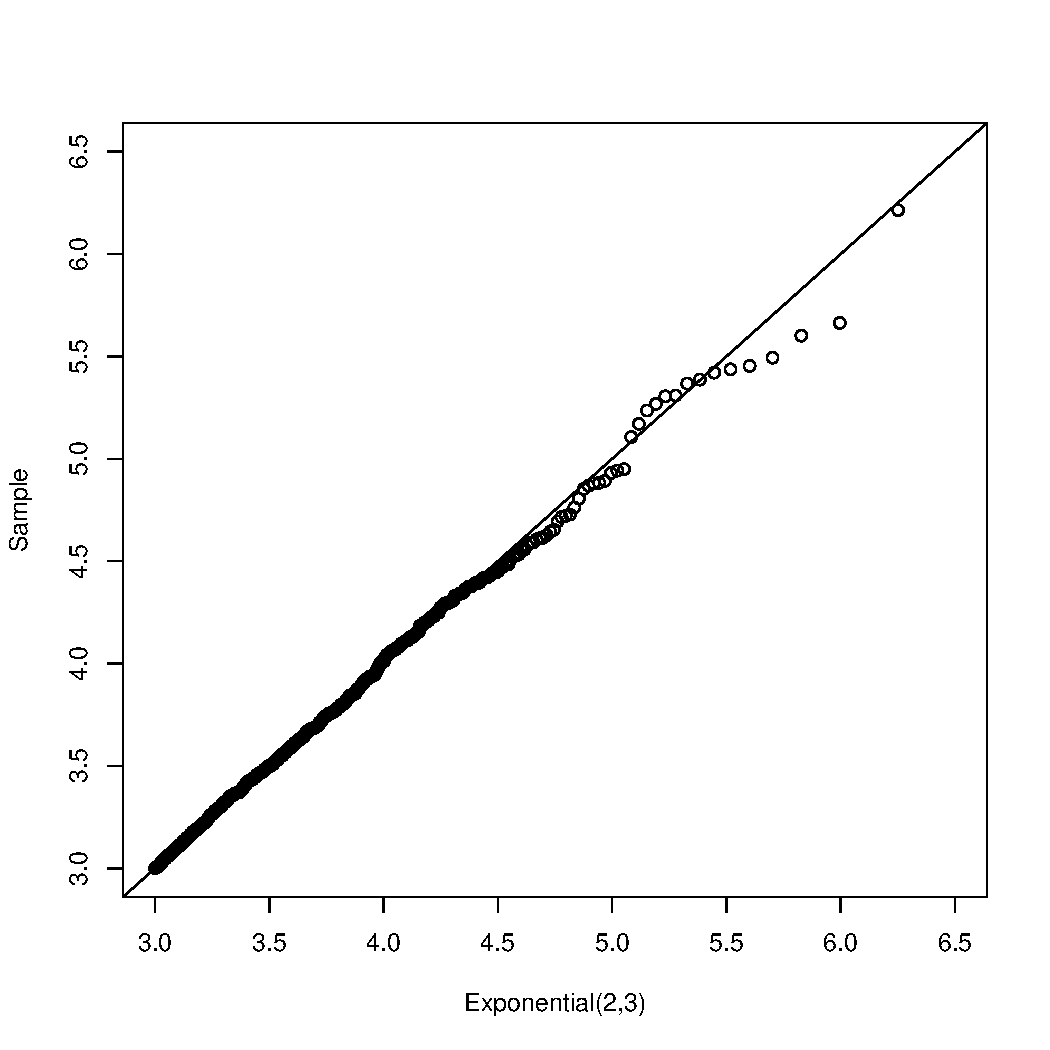
\includegraphics[width=\maxwidth]{figure/qqplot1} 

\end{knitrout}

\caption{Comparison of the randomly generated and theoretical values of the exponential(2,3) distribution. The line represents perfect correspondence.}
\label{exp}
\end{figure}
\clearpage
\item[3.3]We first find the inverse of the Pareto cdf:
$$F^{-1}(u)=exp\left[-\frac{ln(1-u)}{a}+ln(b)\right], u\geq\frac{1}{b}>0,a>0$$
We then use this to generate random sample from a random uniform sample.\\
\begin{knitrout}
\definecolor{shadecolor}{rgb}{0.969, 0.969, 0.969}\color{fgcolor}\begin{kframe}
\begin{alltt}
\hlkwd{require}(VGAM)
r_pareto <- \hlkwd{function}(n, loc, shape) \{
    y <- \hlkwd{c}()
    i <- 1
    \hlkwd{while} (\hlkwd{length}(y) < n) \{
        U <- \hlkwd{runif}(1, min = (1/loc), max = (1))
        x <- \hlkwd{exp}((-1 * \hlkwd{log}(1 - U)/shape) + \hlkwd{log}(loc))
        \hlkwd{if} (x > loc) \{
            y[i] <- x
            i <- i + 1
        \}
    \}
    \hlkwd{return}(y)
\}
x <- \hlkwd{r_pareto}(1000, 2, 2)
ppdf <- \hlkwd{function}(x, a, b) \{
    (a * (b^a))/(x^(a + 1))
\}
\end{alltt}
\end{kframe}
\end{knitrout}

The histogram of the Pareto sample with a density curve from the actual Pareto distribution is in figure \ref{pareto}.
\begin{figure}
\begin{knitrout}
\definecolor{shadecolor}{rgb}{0.969, 0.969, 0.969}\color{fgcolor}
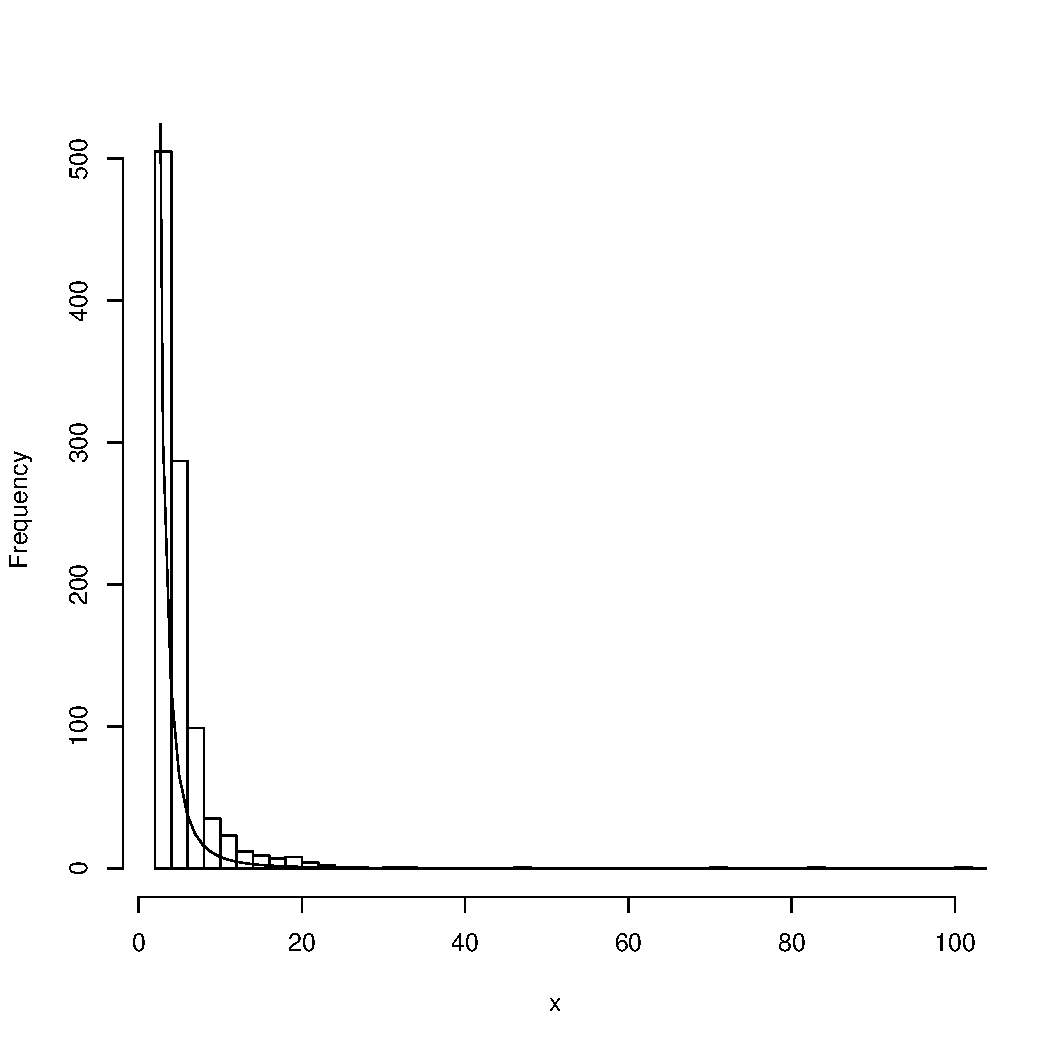
\includegraphics[width=\maxwidth]{figure/plotPareto} 

\end{knitrout}

\caption{Sample from the Pareto generator with the theoretical density overlaid}
\label{pareto}
\end{figure}
\clearpage

\item[3.4] Since I could not find a unique inverse to the Raleigh CDF I will use the accept/reject method.  I will choose $g(y) \sim$ Exponential ($\beta=\sigma^2$).  
$$u< \frac{f(y)}{cg(y)}=\frac{\frac{x}{\sigma^2}e^{-x^2/2\sigma^2}}{\frac{c}{\sigma^2}e^{-x/\sigma^2}}=\frac{xexp(\frac{-x^2-2x}{\sigma^2})}{C}$$
The constant $c$ will change depending on the value of $\sigma$ chosen and therefore it will be useful to have a function which sets $C$ based on $\sigma$.  The maximum of the above function over the support $x\geq0,\sigma>0$ can be determined with some calculus to be:\\
$$x=\frac{\sqrt{1+4\sigma^2}}{2}$$
Several histograms with their associated theoretical modes and the number of random uniform variables required to produce a sample of 1000 are shown in figure \ref{ral}.  As can ebe seen in the above equation this generator becomes increasingly inefficient as $\sigma$ grows.\\  
\begin{knitrout}
\definecolor{shadecolor}{rgb}{0.969, 0.969, 0.969}\color{fgcolor}\begin{kframe}
\begin{alltt}
r_ral <- \hlkwd{function}(n, sigma) \{
    x <- \hlkwd{c}()
    i <- 1
    j <- 1
    s2 <- sigma^2
    c <- (1 + \hlkwd{sqrt}(1 + 4 * sigma^2))/2
    \hlkwd{while} (\hlkwd{length}(x) < n) \{
        u <- \hlkwd{runif}(1)
        y <- \hlkwd{rexp}(1, rate = (1/(sigma^2)))
        j <- j + 1
        \hlkwd{if} (u < ((y * (\hlkwd{exp}((-1 * y^2 + 2 * y)/(2 * s2))))/c)) \{
            x[i] <- y
            i <- i + 1
        \}
    \}
    \hlkwd{return}(\hlkwd{list}(x, j))
\}
r_2 <- \hlkwd{r_ral}(1000, 2)
r_4 <- \hlkwd{r_ral}(1000, 4)
r_6 <- \hlkwd{r_ral}(1000, 6)
r_8 <- \hlkwd{r_ral}(1000, 8)
\end{alltt}
\end{kframe}
\end{knitrout}

\begin{figure}
\begin{knitrout}
\definecolor{shadecolor}{rgb}{0.969, 0.969, 0.969}\color{fgcolor}
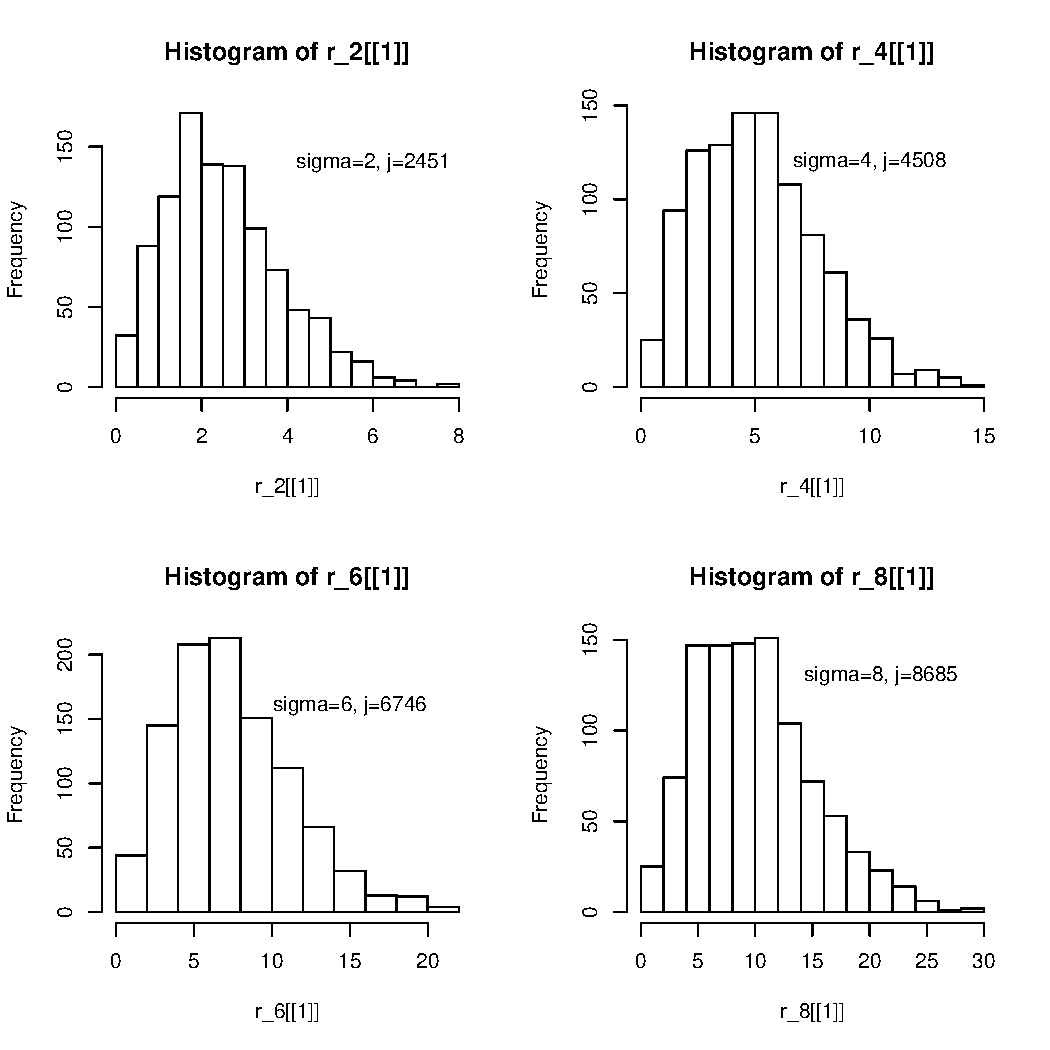
\includegraphics[width=\maxwidth]{figure/plotral} 

\end{knitrout}

\caption{Several Raleigh distributions, the expected modes (sigma) and the number of random samples needed to generate 1000 numbers (j).}
\label{ral}
\end{figure}
\clearpage

\item[3.8] If Z $\sim$ Normal$(\mu,\sigma^2)$ then $e^Z\sim$Lognormal($\mu=e^{\mu+(\sigma^2/2)}, \sigma^2=e^{2(\mu+\sigma^2)}-e^{2\mu+\sigma^2})$. Therefore to get a lognormal($\mu,\sigma^2$) we will need to generate a Z$\sim$Normal and return $e^Z$.  Figure \ref{lnorm} shows the random sample generated from a lognormal(0,1) distribution and the theoretical density.\\
\begin{knitrout}
\definecolor{shadecolor}{rgb}{0.969, 0.969, 0.969}\color{fgcolor}\begin{kframe}
\begin{alltt}
r_lnorm <- \hlkwd{function}(n, mu, sigma2) \{
    x <- \hlkwd{rnorm}(n, mu, sigma2)  \hlcom{#mu+sigma2/2,2*(mu+sigma2)+\hlkwd{log}(1-\hlkwd{exp}(-sigma2)))}
    y <- \hlkwd{exp}(x)
    \hlkwd{return}(y)
\}
l <- \hlkwd{r_lnorm}(1000, 0, 1)
\end{alltt}
\end{kframe}
\end{knitrout}

\begin{figure}
\begin{knitrout}
\definecolor{shadecolor}{rgb}{0.969, 0.969, 0.969}\color{fgcolor}
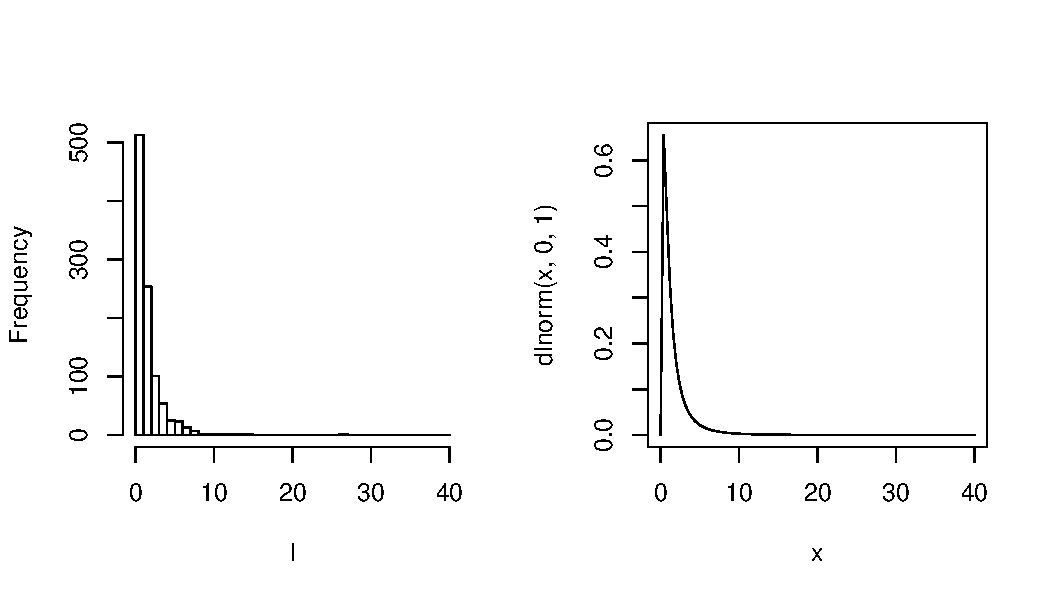
\includegraphics[width=\maxwidth]{figure/lnormplot} 

\end{knitrout}

\caption(A histogram of the randomly generated lognormal sample and the theoretical density of the same distribution)
\label(lnorm)
\end{figure}

\item[3.9] The rescaled Epanechnikov distribution can be simulated with:
\begin{knitrout}
\definecolor{shadecolor}{rgb}{0.969, 0.969, 0.969}\color{fgcolor}\begin{kframe}
\begin{alltt}
r_ekov <- \hlkwd{function}(n) \{
    x <- \hlkwd{c}()
    i <- 1
    \hlkwd{while} (\hlkwd{length}(x) < n) \{
        u1 <- \hlkwd{runif}(1, min = -1, max = 1)
        u2 <- \hlkwd{runif}(1, min = -1, max = 1)
        u3 <- \hlkwd{runif}(1, min = -1, max = 1)
        x[i] <- \hlkwd{ifelse}(u3 >= u2 && u3 >= u1, u2, u3)
        i = i + 1
    \}
    \hlkwd{return}(x)
\}
e <- \hlkwd{r_ekov}(1000)
\end{alltt}
\end{kframe}
\end{knitrout}

The histogram and density estimate are shown in figure \ref{epi}.\\
\begin{figure}
\begin{knitrout}
\definecolor{shadecolor}{rgb}{0.969, 0.969, 0.969}\color{fgcolor}
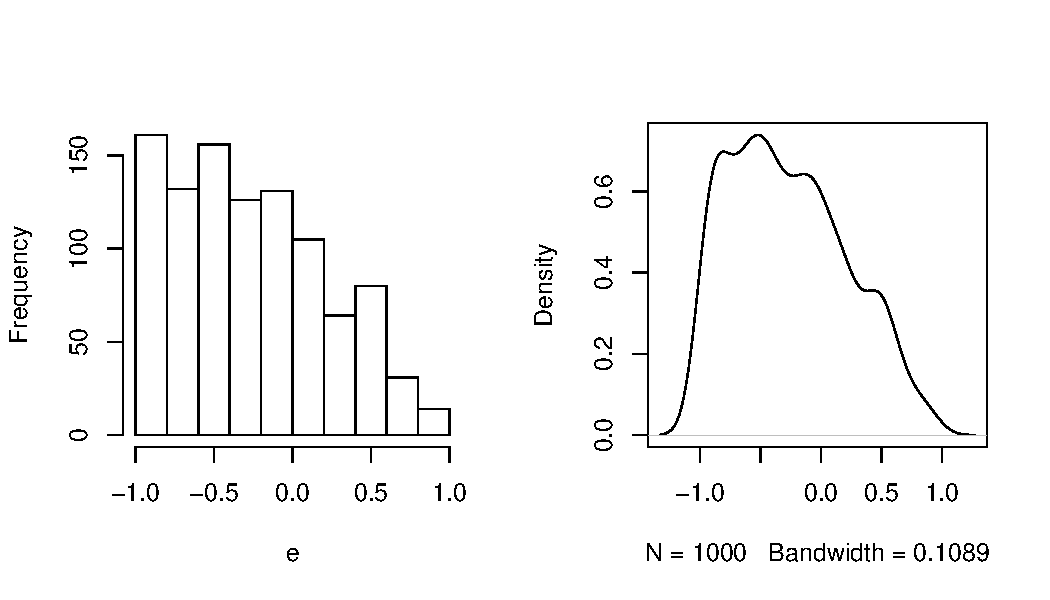
\includegraphics[width=\maxwidth]{figure/plotek} 

\end{knitrout}

\caption{Histogram of the randomly generated Epanechnikov distribution and a corresponding density estimate}
\label{epi}
\end{figure}

\item[3.11]  Mixture of Normal(0,1) and Normal(3,1):\\
\begin{knitrout}
\definecolor{shadecolor}{rgb}{0.969, 0.969, 0.969}\color{fgcolor}\begin{kframe}
\begin{alltt}
rlocmix <- \hlkwd{function}(n, l1, l2, p1) \{
    loc <- \hlkwd{sample}(\hlkwd{c}(l1, l2), size = n, replace = TRUE, prob = \hlkwd{c}(p1, 1 - p1))
    x <- \hlkwd{rnorm}(n, loc, 1)
    \hlkwd{return}(x)
\}
m <- \hlkwd{rlocmix}(1000, 0, 3, 0.75)
m2 <- \hlkwd{rlocmix}(1000, 0, 3, 0.5)
\end{alltt}
\end{kframe}
\end{knitrout}

Based on the results of figure \ref{nmix}, and some simple logic, I would conjecture that p near 0 or 1 would produce a unimodal distriution with skew whereas a p near 0.5 would produce a bimodal distribution.\\
\begin{figure}
\begin{knitrout}
\definecolor{shadecolor}{rgb}{0.969, 0.969, 0.969}\color{fgcolor}
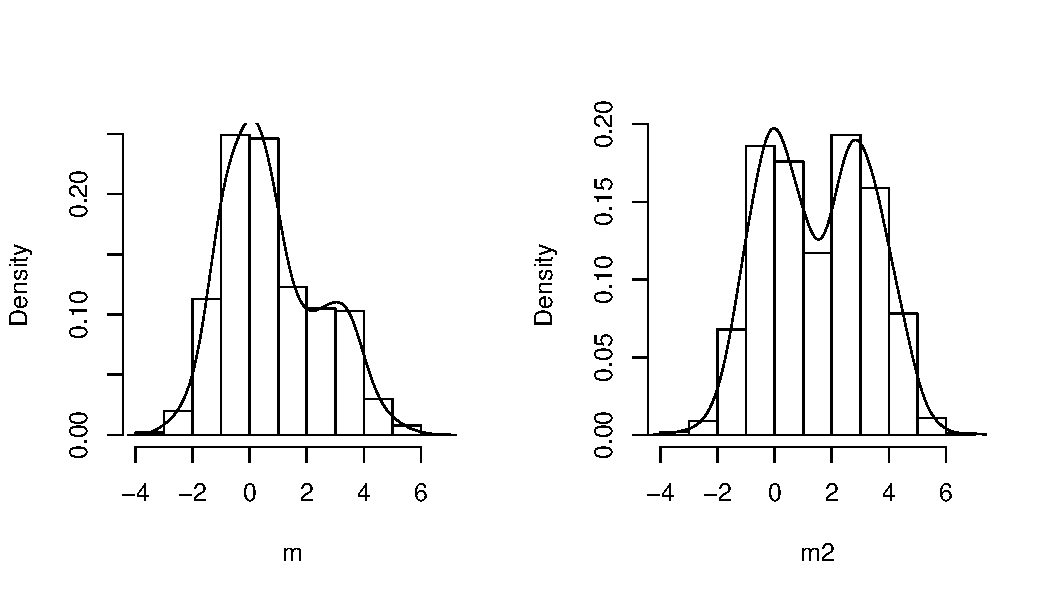
\includegraphics[width=\maxwidth]{figure/mplot} 

\end{knitrout}

\caption{Two normal location mixtures one with p=.75 (left) and one with p=.5 (right).  I would conjecture that p near 0 or 1 would produce a unimodal distriution with skew whereas a p near .5 would produce a bimodal distribution.}
\label{nmix}
\end{figure}

\item[3.12] Continuous mixture of Exponential($\Lambda$) with $\Lambda\sim$Gamma($r,\beta$).\\
\begin{knitrout}
\definecolor{shadecolor}{rgb}{0.969, 0.969, 0.969}\color{fgcolor}\begin{kframe}
\begin{alltt}
lam <- \hlkwd{rgamma}(1000, shape = 2, rate = 4)
x <- \hlkwd{rexp}(1000, rate = lam)
\hlkwd{rm}(list = \hlkwd{ls}())
\end{alltt}
\end{kframe}
\end{knitrout}


\item[3.14] This is taken right from example 3.18, results are in figure \ref{mvplot}:\\
\begin{knitrout}
\definecolor{shadecolor}{rgb}{0.969, 0.969, 0.969}\color{fgcolor}\begin{kframe}
\begin{alltt}
rmvn.Choleski <- \hlkwd{function}(n, mu, Sigma) \{
    d <- \hlkwd{length}(mu)
    Q <- \hlkwd{chol}(Sigma)
    Z <- \hlkwd{matrix}(\hlkwd{rnorm}(n * d), nrow = n, ncol = d)
    X <- Z %*% Q + \hlkwd{matrix}(mu, n, d, byrow = TRUE)
    X
\}

mu <- \hlkwd{c}(0, 1, 2)
Sigma <- \hlkwd{matrix}(\hlkwd{c}(1, -0.5, 0.5, -0.5, 1, -0.5, 0.5, -0.5, 1), 3, 3)
X <- \hlkwd{rmvn.Choleski}(200, mu, Sigma)
\end{alltt}
\end{kframe}
\end{knitrout}

\begin{figure}
\begin{knitrout}
\definecolor{shadecolor}{rgb}{0.969, 0.969, 0.969}\color{fgcolor}
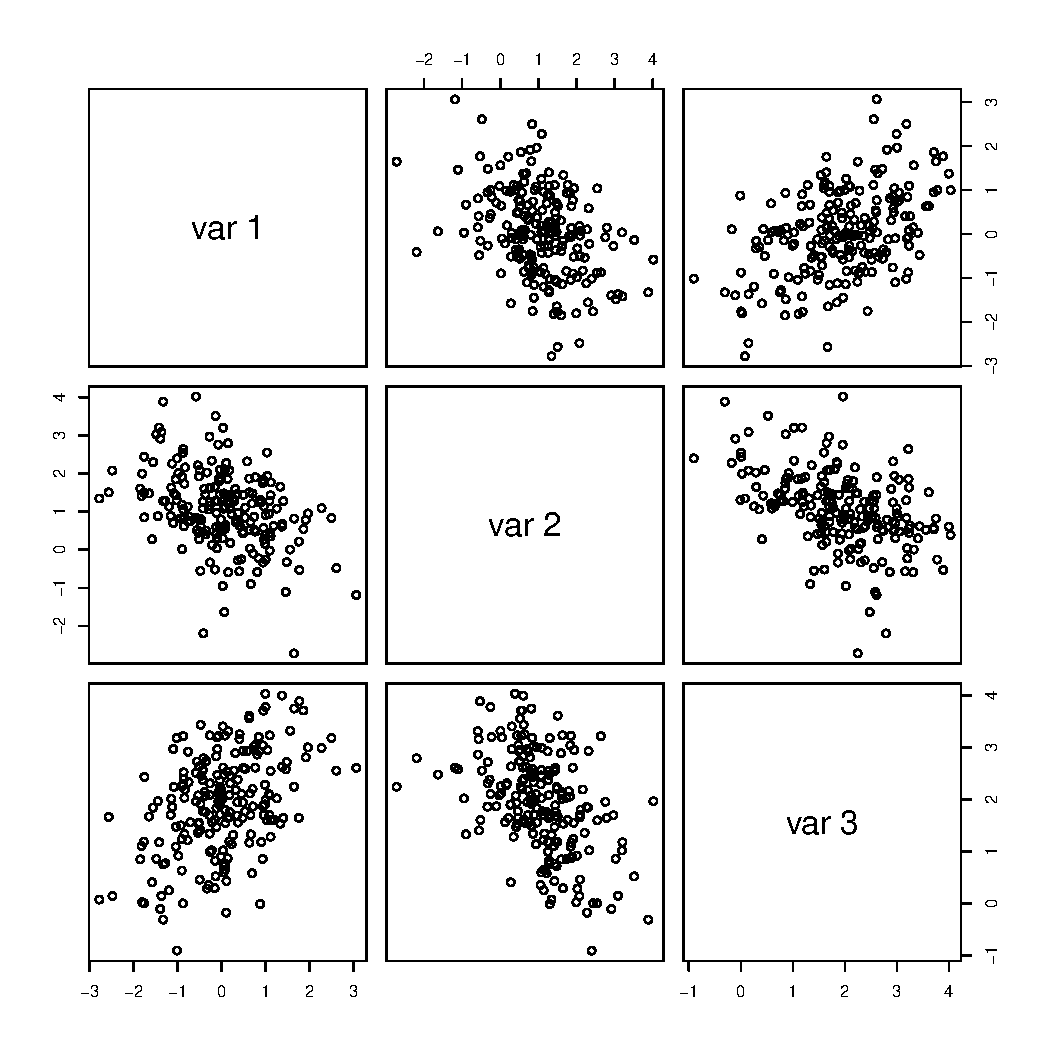
\includegraphics[width=\maxwidth]{figure/pplot} 

\end{knitrout}

\caption{The scatterplot matrix from the multivariable normal sample relfect the covariance matrix ($\Sigma$) used to generate them.}
\label{mvplot}
\end{figure}

\item[3.18]  Simulate the Weishart distribution:\\
\begin{knitrout}
\definecolor{shadecolor}{rgb}{0.969, 0.969, 0.969}\color{fgcolor}\begin{kframe}
\begin{alltt}
\hlcom{# generate lower triangular N(0,1) matrix T with d=5}
T <- \hlkwd{matrix}(\hlkwd{rnorm}(15), 5, 5)
T[\hlkwd{upper.tri}(T)] <- 0
i <- 1:5
d <- \hlkwd{sqrt}(\hlkwd{rchisq}(\hlkwd{length}(i), 6 - i + 1))
\hlkwd{diag}(T) <- d
T  \hlcom{#lower triangular matrix of \hlkwd{N}(0,1)}
\end{alltt}
\begin{verbatim}
##         [,1]    [,2]    [,3]   [,4]  [,5]
## [1,]  2.6822  0.0000  0.0000 0.0000 0.000
## [2,]  0.8588  1.8874  0.0000 0.0000 0.000
## [3,] -1.7585 -1.8231  1.2723 0.0000 0.000
## [4,] -0.4917  1.8010 -0.1232 1.1242 0.000
## [5,]  0.2302 -0.2214 -0.5310 0.2302 1.124
\end{verbatim}
\begin{alltt}
A <- T %*% \hlkwd{t}(T)
A
\end{alltt}
\begin{verbatim}
##         [,1]    [,2]    [,3]    [,4]    [,5]
## [1,]  7.1944  2.3036 -4.7169 -1.3189  0.6175
## [2,]  2.3036  4.2999 -4.9512  2.9770 -0.2202
## [3,] -4.7169 -4.9512  8.0348 -2.5755 -0.6768
## [4,] -1.3189  2.9770 -2.5755  4.7646 -0.1877
## [5,]  0.6175 -0.2202 -0.6768 -0.1877  1.6998
\end{verbatim}
\begin{alltt}
\hlcom{# make symmetric sigma matrix}
\hlkwd{require}(Matrix)
sigma <- \hlkwd{forceSymmetric}(\hlkwd{matrix}(\hlkwd{c}(1, 0, 0, 0, 0, 0.5, 1, 0, 0, 0, 0.5, 0.5, 1, 
    0, 0, 0.5, 0.5, 0.5, 1, 0, 0.5, 0.5, 0.5, 0.5, 1), 5, 5))
l <- \hlkwd{chol}(sigma)
x <- \hlkwd{t}(l) %*% A %*% l
x
\end{alltt}
\begin{verbatim}
## 5 x 5 Matrix of class "dgeMatrix"
##        [,1]   [,2]    [,3]   [,4]    [,5]
## [1,] 7.1944  5.592  0.4109  2.257  3.5691
## [2,] 5.5922  7.018 -1.2231  4.364  3.2417
## [3,] 0.4109 -1.223  1.9931 -1.209 -0.2438
## [4,] 2.2567  4.364 -1.2092  4.073  1.8648
## [5,] 3.5691  3.242 -0.2438  1.865  2.7662
\end{verbatim}
\begin{alltt}
\hlkwd{rm}(list = \hlkwd{ls}())
\end{alltt}
\end{kframe}
\end{knitrout}


\item[3.19]  Random symmetric walk, figure \ref{walk} shows the results:\\
\begin{knitrout}
\definecolor{shadecolor}{rgb}{0.969, 0.969, 0.969}\color{fgcolor}\begin{kframe}
\begin{alltt}
A <- 10
trace <- \hlkwd{vector}()
i <- 1
\hlkwd{while} (A < 20 && A > 0) \{
    win <- \hlkwd{sample}(\hlkwd{c}(-1, 1), size = 1, prob = \hlkwd{c}(0.5, 0.5))
    trace[i] <- A  \hlcom{#place the trace before updating A to get \hlkwd{A}(0)}
    A <- A + win
    i <- i + 1
\}
A
\end{alltt}
\begin{verbatim}
## [1] 0
\end{verbatim}
\begin{alltt}
trace
\end{alltt}
\begin{verbatim}
##   [1] 10 11 12 11 10 11 10 11 10 11 12 13 14 13 14 15 16 15 16 15 14 15 14
##  [24] 13 14 13 12 11 12 11 12 11 12 11 12 13 14 15 16 17 18 17 16 17 18 17
##  [47] 18 17 18 17 18 19 18 17 18 17 18 17 16 15 16 17 16 17 16 15 14 15 16
##  [70] 15 14 13 12 11 12 11 10 11 12 11 12 11 10 11 10 11 10 11 10 11 10 11
##  [93] 12 11 10  9  8  7  6  5  4  5  4  5  6  7  6  7  8  7  8  9 10 11 12
## [116] 11 12 13 12 13 12 11 10  9  8  9  8  7  8  7  8  7  6  5  6  7  8  9
## [139]  8  7  6  7  8  7  8  9  8  7  8  9 10  9 10 11 10  9  8  9  8  7  8
## [162]  7  6  7  8  7  6  7  6  5  6  7  8  7  6  5  6  5  6  7  8  9 10  9
## [185]  8  7  6  5  4  5  6  5  6  5  6  5  6  7  6  7  6  7  8  7  8  9 10
## [208]  9 10 11 12 11 10  9  8  9  8  9  8  9 10 11 10  9  8  7  6  5  4  3
## [231]  4  5  6  5  4  3  2  3  4  3  4  5  6  7  8  9 10 11 12 11 12 13 14
## [254] 15 14 15 14 15 14 13 12 13 12 11 10  9 10  9 10 11 10  9  8  7  8  7
## [277]  8  7  8  7  8  7  6  5  4  5  4  5  6  5  4  5  4  5  4  5  6  5  6
## [300]  5  6  7  6  7  8  7  8  7  8  7  8  9  8  7  6  5  4  3  2  3  2  1
\end{verbatim}
\begin{alltt}
t <- 1:\hlkwd{length}(trace)
\end{alltt}
\end{kframe}
\end{knitrout}

\begin{figure}
\begin{knitrout}
\definecolor{shadecolor}{rgb}{0.969, 0.969, 0.969}\color{fgcolor}
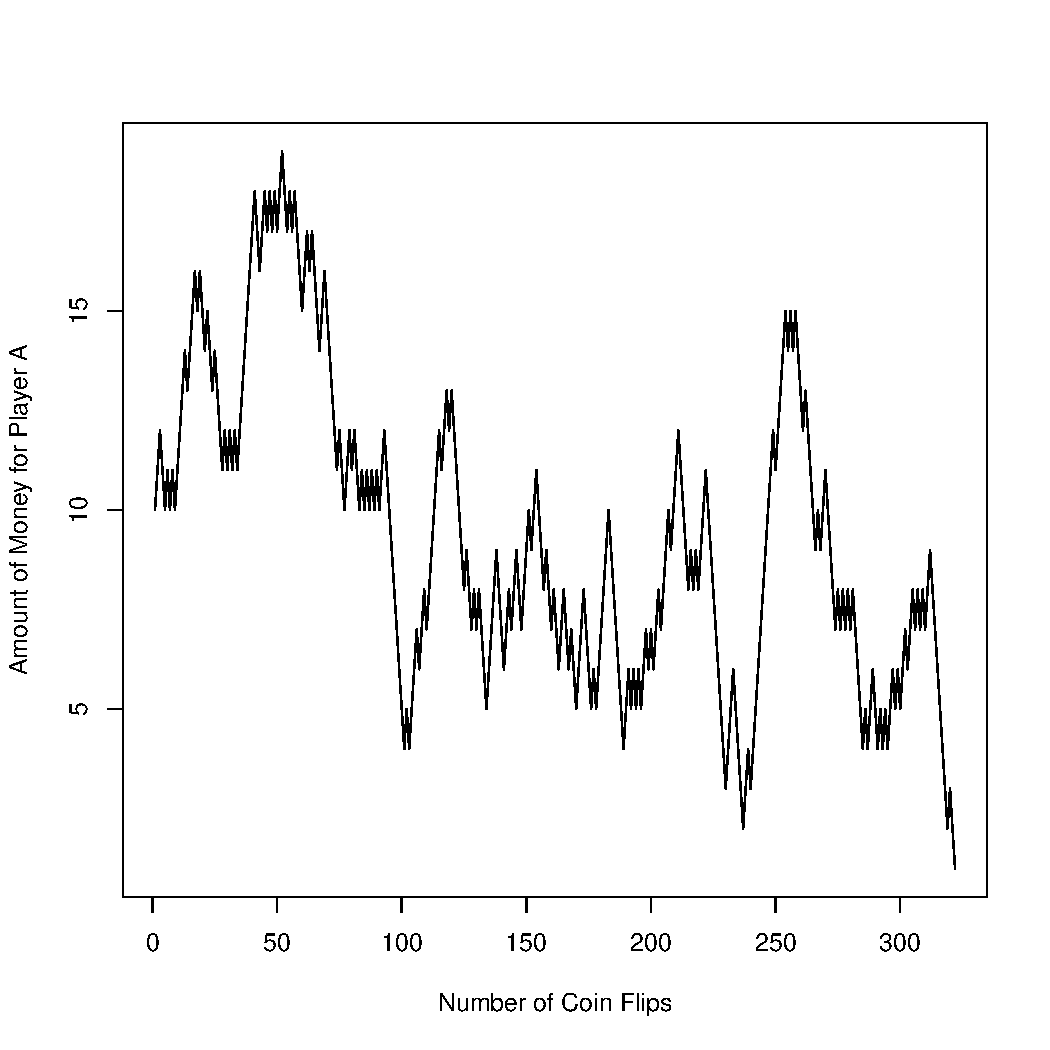
\includegraphics[width=\maxwidth]{figure/walkplot} 

\end{knitrout}

\caption{Plot of the random symmetric walk.}
\label{walk}
\end{figure}
\end{itemize}
\end{document}
